%************************************************
\chapter{A basic introduction to Learning-to-Rank}
Different definitions of Learning-to-Rank exist. In general, all ranking methods that use machine learning technologies to solve the problem of ranking are called Learning-to-Rank methods. Figure \ref{fig:discriminative_training} describes the general process of machine learning. It shows training elements from an input space that are mapped to an output space using a model such that the difference between the actual labels of the training elements and the labels predicted with with the model are minimal in terms of a loss function.
\begin{figure}[!h]
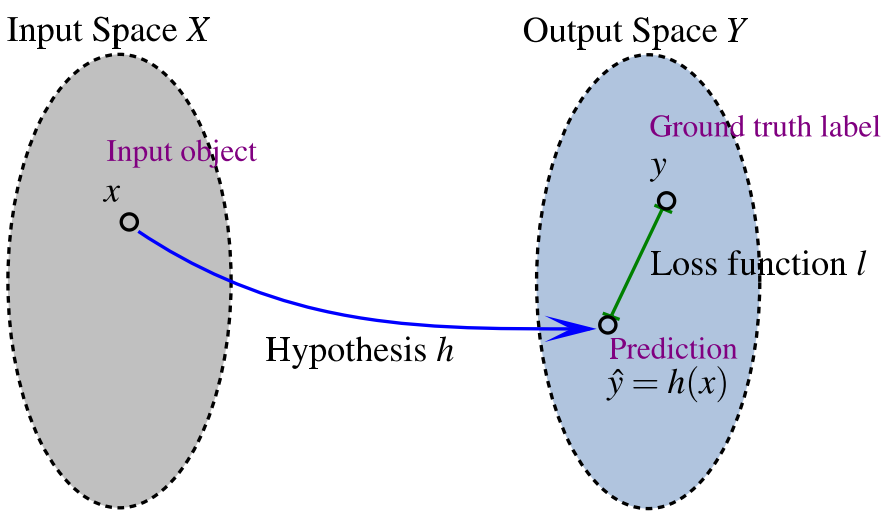
\includegraphics[scale=0.26]{gfx/descriminative_training}
\caption{Machine learning framework for Learning-to-Rank, obtained from Liu \cite{Liu2007}}
\label{fig:discriminative_training}
\end{figure}\\
Liu \cite{Liu2007} proposes a more narrow definition and only considers ranking methods to be a Learning-to-Rank method when it is \emph{feature based} and uses \emph{discriminative training}, which are itself defined as follows:
\begin{description}
\item[Feature Based]{means that all documents under investigation are represented by feature vectors. Those feature vectors reflect the relevance of the documents to the query, or the importance of the document in itself.}
\item[Discriminative Training]{means that the learning process can be well described by the four components of discriminative learning. That is, a Learning-to-Rank method has its own \emph{input space}, \emph{output space}, \emph{hypothesis space}, and \emph{loss function}, like the machine learning process described by Figure \ref{fig:discriminative_training}. \emph{Input space}, \emph{output space}, \emph{hypothesis space}, and \emph{loss function} are hereby defined as follows:
	\begin{description}
	\item[Input Space]{contains the objects under investigation. Usually objects are represented by feature vectors, extracted according to different applications.}
	\item[Output Space]{contains the learning target with respect to the input objects.}
	\item[Hypothesis Space]{defines the class of functions mapping the input space to the output space. The functions operate on the feature vectors of the input object, and make predictions according to the format of the output space.}
	\item[Loss Function]{in order to learn the optimal hypothesis, a training set is usually used, which contains a number of objects and their ground truth labels, sampled from the product of the input and output spaces.}
	\end{description}
	}
\end{description}


Figure \ref{fig:ltr_framework} shows how the machine learning process as described in Figure \ref{fig:discriminative_training} typically takes place in a ranking scenario. A set of queries $q_i$ with $n > i > 1$, the documents associated with these queries which are represented by feature vector $x_i$, and the relevant judgements of those documents $y_i$ are used together to train a model $h$. Model $h$ can after training be used to predict a ranking of the documents $y_i$, such the difference between the document rankings predicted by $h$ and the actual optimal rankings based on $y_i$ is minimal in terms of a loss function.
\begin{figure}[!h]
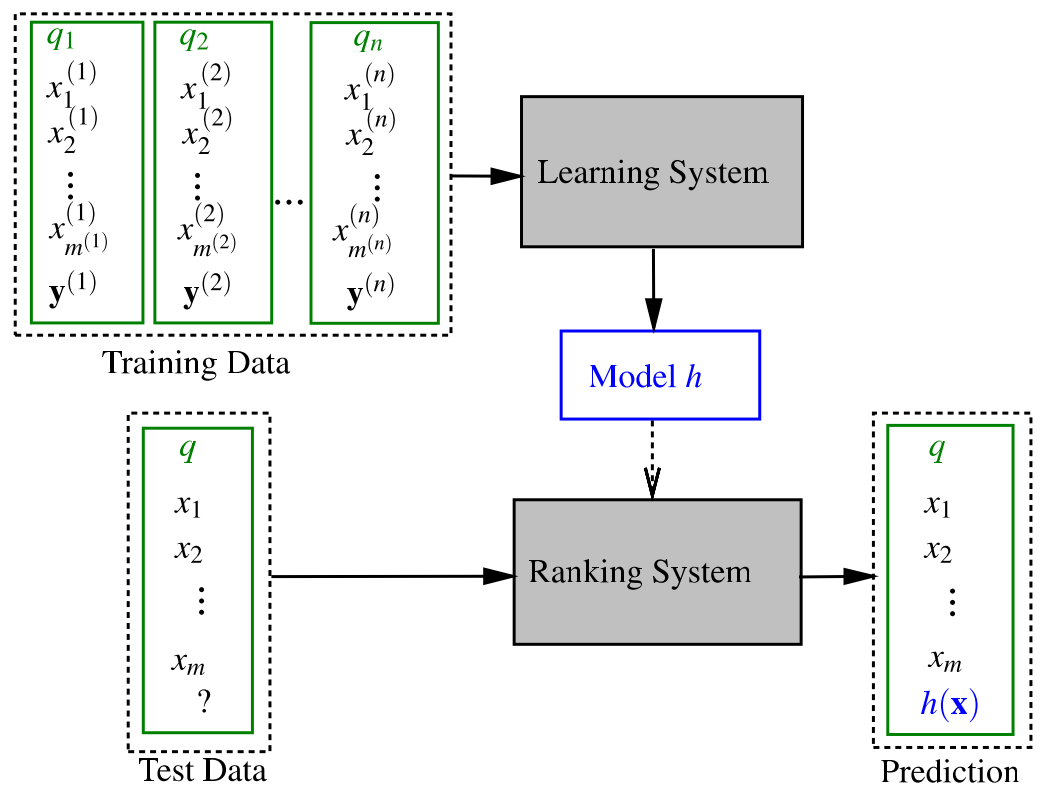
\includegraphics[scale=0.25]{gfx/ltr_framework}
\caption{A typical Learning-to-Rank setting, obtained from Liu \cite{Liu2007}}
\label{fig:ltr_framework}
\end{figure}\\

The predictions and the loss function might either be defined for:
\begin{enumerate}
\item the relevance of a single document
\item the classification of the most relevant document out of a document-pair
\item the ranking of documents directly
\end{enumerate}
These three approaches are in literature respectively called the pointwise approach, the pairwise approach and the listwise approach. These three approaches to Learning-to-Rank will be described in more detail further on in this part.

\chapter{Evaluating a ranking}
Evaluation metrics have long been studied in the field of information retrieval. First in the form of evaluation of unranked retrieval sets and later, when the information retrieval field started focussing more on ranked retrieval, in the form of ranked retrieval evaluation. In the succeeding section several frequently used evaluation metrics for ranked results will be described.\\

No single evaluation metric that we are going to describe is indisputably better or worse than any of the other metrics. Different benchmarking settings have used different evaluation metrics. Metrics introduced in this section will be used to express the evaluation results in the Benchmark Results part of this thesis.
\section{Normalized Discounted Cumulative Gain}
Cumulative gain, or its predecessor discounted cumulative gain and normalized discounted cumulative gain, is one of the most widely used measures for effectiveness of ranking methods.
\subsection{Discounted Cumulative Gain}
There are two definitions of \ac{DCG} used in practice. \ac{DCG} at position $p$ was originally defined by J{\"a}rvelin and Kek{\"a}l{\"a}inen \cite{Jarvelin2002} as\\

$DCG_p = \sum\nolimits_{i=1}^p \frac{rel_i-1}{log_2(i+1)}$\\

with $rel_i$ the graded relevance of the result at position $i$. The idea is that highly relevant documents that appear lower in a search result should be penalized (discounted). This discounting is done by reducing the graded relevance  logarithmically proportional to the position of the result.\\

Burges et al. \cite{Burges2005} proposed an alternative definition of \ac{DCG} that puts stronger emphasis on document relevance\\

$DCG_p = \sum\nolimits_{i=1}^p \frac{2^{rel_i-1}}{log_2(i+1)}$\\


\subsection{Normalized Discounted Cumulative Gain}
\ac{nDCG} normalizes the \ac{DCG} metric to a value in the [0,1] interval by dividing by the \ac{DCG} value of the optimal rank. This optimal rank is obtained by sorting documents on relevance for a given query. The definition of \ac{nDCG} can be written down mathematically as\\

$nDCG_p = \frac{DCG_p}{IDCG_p}$\\

Table \ref{tab:example_calculation_nDCG} shows an example calculation for \ac{nDCG} for both the J{\"a}rvelin and Kek{\"a}l{\"a}inen \cite{Jarvelin2002} and Burges et al. \cite{Burges2005} version of \ac{DCG}.

\begin{table}[!h]
\begin{tabular}{llllllllllll}
 & \multicolumn{10}{c}{Rank} &  \\ 
\cline{2-11}
 & 1 & 2 & 3 & 4 & 5 & 6 & 7 & 8 & 9 & 10 & Sum \\ 
\hline
\hline
rel(i) & 10 & 7 & 6 & 8 & 9 & 5 & 1 & 3 & 2 & 4 &  \\
\hline
$\frac{2^{rel_i-1}}{log_2(i+1)}$ & 512 & 40.4 & 16 & 55.1 & 99.0 & 5.7 & 0.3 & 1.3 & 0.6 & 2.3 & 732.7 \\
\hline
$\frac{rel_i}{log_2(i+1)}$ & 10 & 4.42 & 3 & 3.45 & 3.48 & 1.78 & 0.33 & 0.95 & 0.6 & 1.16 & 29.17 \\  
\hline
\hline
optimal rank & 10 & 9 & 8 & 7 & 6 & 5 & 4 & 3 & 2 & 1 &  \\
\hline 
$\frac{2^{rel_i-1}}{log_2(i+1)}$ & 512 & 161.5 & 64 & 27.6 & 12.4 & 5.7 & 2.7 & 1.3 & 0.6 & 0.2 & 788.0 \\
\hline
$\frac{rel_i}{log_2(i+1)}$ & 10 & 5.68 & 4 & 3.01 & 2.32 & 1.78 & 1.33 & 0.95 & 0.6 & 0.29 & 29.96 \\   
\hline
 &  &  &  &  &  &  &  &  &  &  &  \\
 & \multicolumn{10}{c}{J{\"a}rvelin and Kek{\"a}l{\"a}inen \cite{Jarvelin2002} \ac{nDCG} = $\frac{29.17}{29.96} = 0.97$} &  \\  
 & \multicolumn{10}{c}{Burges \cite{Burges2005} et al. \ac{nDCG} = $\frac{732.7}{788.0} = 0.93$} &  \\ 
\end{tabular}
\caption{Example calculation for \ac{nDCG}}
\label{tab:example_calculation_nDCG}
\end{table}
\section{Expected Reciprocal Rank}
\ac{ERR} \cite{Chapelle2009} was designed based on the observation that \ac{nDCG} is based on the false assumption that the usefulness of a document at rank $i$ is independent of the usefulness of the documents at rank less than $i$. \ac{ERR} is based on the reasoning that users are likely to stop exploring the result list once they have found a document that satisfied their information need. The \ac{ERR} metric is defined as the expected reciprocal length of time that the user will take to find a relevant document. \ac{ERR} is formally defined as\\

$ERR = \sum\nolimits_{r=1}^n \frac{1}{r} \prod\nolimits_{i=1}^{r-1}(1-R_i)R_i$\\

where the product sequence part of the formula represents the chance that the user will stop at position $r$.\\
An algorithm to compute \ac{ERR} is shown in Listing \ref{lst:err}. The algorithm requires relevance grades $g_i$, $1 \le i \le n$ and mapping function $R$ that maps relevance grades to probability of relevance.
\begin{lstlisting}[caption={Algorithm to compute the ERR metric, obtained from \cite{Chapelle2009}}, label={lst:err},language=Ada]
p <- 1, ERR <- 0
for r=1 to n do
	R <- R(g[r])
	ERR <- ERR + p * R/r
	p <- p * (1-R)
end for
return ERR
\end{lstlisting}
\section{Mean Average Precision}
\ac{AP} \cite{Zhu2004} is an often used binary relevance judgement based metric that can be seen as a trade-off between precision and recall that is defined as\\

$AP = \frac{\sum\nolimits_{k=1}^{n}Precision(k)*relevance(k)}{\text{number of relevant docs}}$\\

With $k$ being the positions in the result set between 1 and $n$. Table \ref{tab:example_calculation_AP} provides an example calculation of average precision where de documents at positions 1, 5, 6 and 8 in the ranking are relevant.
\ac{MAP} is the average \ac{AP} for a set of queries.\\

$MAP = \frac{\sum\nolimits_{q=1}^{Q}AP(q)}{Q}$\\

\begin{table}
\begin{tabular}{lllllllllllll}
 & \multicolumn{10}{c}{Rank} &  & Sum \\ 
\cline{2-11}
 & 1 & 2 & 3 & 4 & 5 & 6 & 7 & 8 & 9 & 10 &  &  \\ 
\hline
$r_i$ & 1 & 0 & 0 & 0 & 1 & 1 & 0 & 1 & 0 & 0 &  &  \\ 
P@$i$ & 1 &  &  &  & 0.4 & 0.5 &  & 0.5 &  &  &  & 2.4 \\ 
\hline
 &  &  &  &  &  &  &  &  &  & /\#Relevant docs & = & 7 \\ 
 &  &  &  &  &  &  &  &  &  & AP@10 & = & 0.34 \\ 
\end{tabular}
\caption{Average Precision example calculation. The number of relevant documents \emph{R} is assumed to be seven.}
\label{tab:example_calculation_AP}
\end{table}

\chapter{Approaches to Learning-to-Rank}
\section{Pointwise Approach}
The pointwise approach can be seen as the most straightforward way of using machine learning for ranking. Pointwise Learning-to-Rank methods directly apply machine learning methods to the ranking problem by observing each document in isolation. They can be subdivided in the following approaches:
	\begin{enumerate}
	\item regression-based, which estimate the relevance of a considered document using a regression model.
	\item classification-based, which classify the relevance category of the document using a classification model.
	\item ordinal regression-based, which classify the relevance category of the document using a classification model in such a way that the order of relevance categories is taken into account. 
	\end{enumerate}
\section{Pairwise Approach}
Pointwise Learning-to-Rank methods have the drawback that they optimise real valued expected relevance, while evaluation metrics like \ac{nDCG} and \ac{ERR} are only impacted by a change in expected relevance when that change impacts a pairwise preference. The pairwise approach solves this drawback of the pointwise approach by regarding ranking as pairwise classification.\\

Aggregating a set of predicted pairwise preferences into the corresponding optimal rank is shown to be a NP-Hard problem \cite{Feldman2012}. An often used solution to this problem is to upper bound the number of classification mistakes by an easy to optimise function \cite{Bartlett2006}.
\section{Listwise Approach}
Listwise ranking optimises the actual evaluation metric. The learner learns to predict an actual ranking itself without using an intermediate step like in pointwise or pairwise Learning-to-Rank. The main challenge in this approach is that most evaluation metrics are not differentiable. \ac{MAP}, \ac{ERR} and \ac{nDCG} are non-differentiable, non-convex and discontinuous functions, what makes them very hard to optimize.\\

Although the properties of \ac{MAP}, \ac{ERR} and \ac{nDCG} are not ideal for direct optimisation, some listwise approaches do focus on direct metric optimisation \cite{Yue2007, Taylor2008, Chapelle2010}. Most listwise approaches work around optimisation of the non-differentiable, non-convex and discontinuous metrics by optimising surrogate cost functions that mimic the behaviour of \ac{MAP}, \ac{ERR} or \ac{nDCG}, but have nicer properties for optimisation. 